%%%%%%%%%%%%%%%%%%%%%%%%%%%%%%%%%%%%%%%%%%%%%%%%
% vim: set fileencoding=utf-8 :                %
% Author: Andre Anjos <andre.anjos@idiap.ch>   %
% Last update: Fri 19 Jun 20:00:00 2015 CEST   %
%%%%%%%%%%%%%%%%%%%%%%%%%%%%%%%%%%%%%%%%%%%%%%%%
\section{Getting Started}

\subsection{Introduction to Version Control Systems}

\begin{frame}
  \frametitle{Version Control}

  \begin{center}
    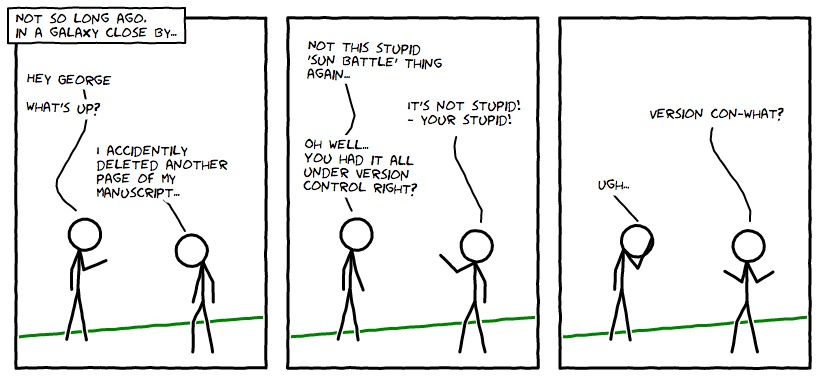
\includegraphics[width=1.0\linewidth]{figures/git-comics}
  \end{center}

\end{frame}

\begin{frame}
  \frametitle{What is Revision Control?}

  \begin{itemize}
    \item Management of changes to documents/code or any sorts of collections
      of information
    \item It is normally done by specialized software packages such as
      \texttt{git}
    \item There are two types:
      \begin{itemize}
        \item Centralized: Revision history is kept on a remote server
        \item Distributed: History is copied with the repository
      \end{itemize}
  \end{itemize}

  \begin{center}
    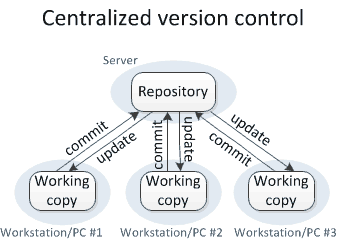
\includegraphics[width=0.45\linewidth]{figures/git-centralized}
    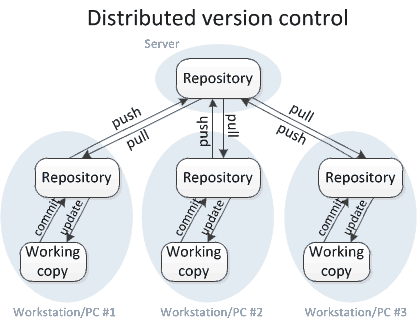
\includegraphics[width=0.45\linewidth]{figures/git-distributed}
  \end{center}

\end{frame}


\begin{frame}
  \frametitle{Why is it necessary?}

  Imagine a world w/o version control:

  \begin{itemize}
    \item You released version 1.0 of your software. It has a bug. Which other
      versions are affected?
    \item When was the last time I touched this file? Which changes did I do?
    \item You introduced a bug on the software: Where is that \textit{fracking}
      backup?
  \end{itemize}

  \begin{alertblock}{It is possible!}
    Actually, the Linux project stayed 11 years w/o version control!

    \vspace{1em}

    This was possible thanks to an ``extremely" organized procedure for
    diff/patching changes that gave birth to what is ``Git" today!
  \end{alertblock}

\end{frame}

\begin{frame}
  \frametitle{About Version Control}

  If you are a graphic or web designer and want to keep every version of an image or layout (which you would most certainly want to), a Version Control System (VCS) is a very wise thing to use. It allows you to:
  
  \begin{itemize}
   \item revert selected files back to a previous state, 
   \item revert the entire project back to a previous state, 
   \item compare changes over time, 
   \item see who last modified something that might be causing a problem, 
   \item who introduced an issue and when, and more. 
  \end{itemize}
\end{frame}

\subsection{Local vs Centralized vs Distributed VCS}

\begin{frame}
  \frametitle{Local Version Control Systems}
  One of the more popular VCS tools was a system called RCS, which is still distributed with many computers today. RCS works by keeping patch sets (that is, the differences between files) in a special format on disk; it can then re-create what any file looked like at any point in time by adding up all the patches.
  \vspace{1em}
  \begin{center}
    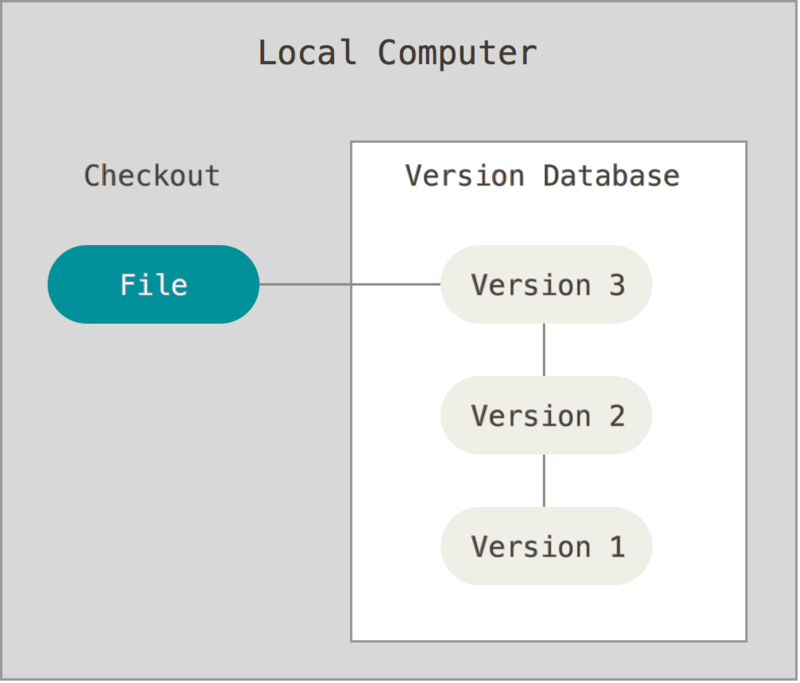
\includegraphics[width=0.5\linewidth]{figures/local}
  \end{center}
\end{frame}


\begin{frame}
  \frametitle{Centralized Version Control Systems (1)}
  The next major issue that people encounter is that they need to collaborate with developers on other systems. To deal with this problem, Centralized Version Control Systems (CVCSs) were developed. These systems (such as CVS, Subversion, and Perforce) have a single server that contains all the versioned files, and a number of clients that check out files from that central place. 
  \vspace{1em}
  \begin{center}
    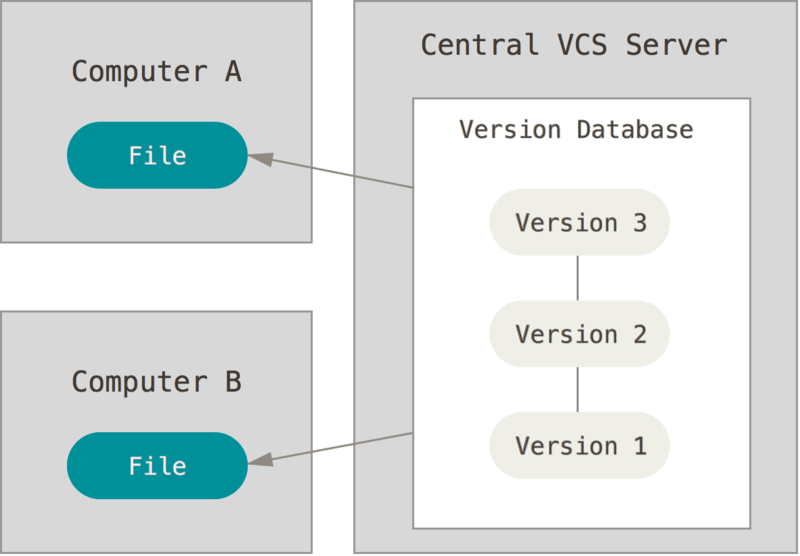
\includegraphics[width=0.5\linewidth]{figures/centralized}
  \end{center}
\end{frame}

\begin{frame}
  \frametitle{Centralized Version Control Systems (2)}
  This setup offers many advantages, especially over local VCSs.
  \begin{itemize}
   \item everyone knows to a certain degree what everyone else on the project is doing.
   \item Administrators have fine-grained control over who can do what, and it's far easier to administer a CVCS than it is to deal with local databases on every client. 
  \end{itemize}
  However, this setup also has some serious downsides:
  \begin{itemize}
   \item If that server goes down for an hour, then during that hour nobody can collaborate at all or save versioned changes to anything they're working on.
   \item If the hard disk the central database is on becomes corrupted, and proper backups haven't been kept, you lose absolutely everything-the entire history of the project.
  \end{itemize}
\end{frame}

\begin{frame}
  \frametitle{Distributed Version Control Systems}
  In a DVCS, such as Git, clients don’t just check out the latest snapshot of the files; rather, they fully mirror the repository, including its full history.
    \vspace{1em}
  \begin{center}
    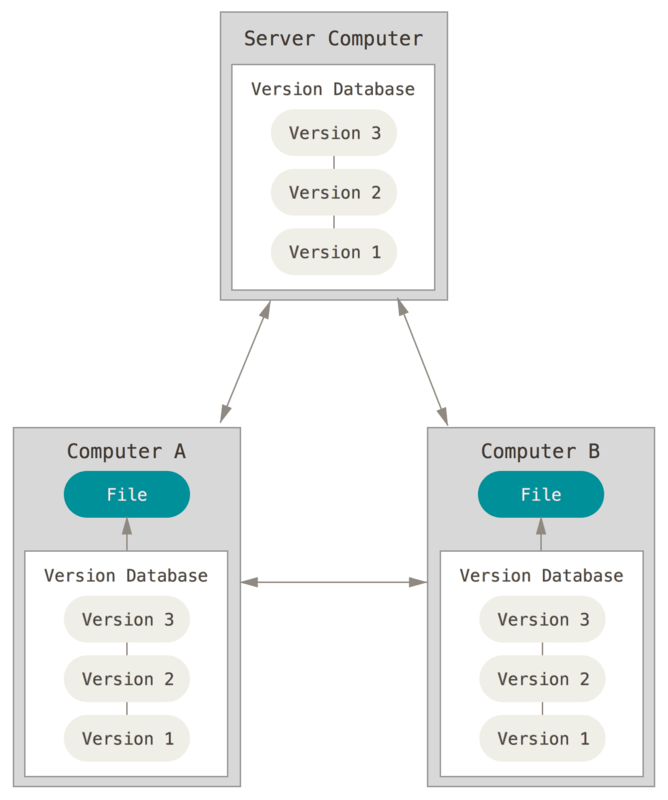
\includegraphics[width=0.5\linewidth]{figures/distributed}
  \end{center}
\end{frame}

\begin{frame}
  \frametitle{Distributed Version Control Systems}
   If any server dies, and these systems were collaborating via that server, any of the client repositories can be copied back up to the server to restore it. Every clone is really a full backup of all the data.
   Furthermore, many of these systems deal pretty well with having several remote repositories they can work with, so you can collaborate with different groups of people in different ways simultaneously within the same project. This allows you to set up several types of workflows that aren’t possible in centralized systems, such as hierarchical models.
\end{frame}

\subsection{Installing git}

\begin{frame}
\frametitle{Installing git}
The first step on the way to using Git is to install it! The directions found in the Git documentation below are pretty thorough and helpful, check them out for the best method of getting Git onto your platform of choice.

 \begin{itemize}
   \item \href{https://git-scm.com/downloads}{Git download page}
   \item \href{https://git-scm.com/book/en/v2/Getting-Started-Installing-Git}{Git installation instructions for each platform}
  \end{itemize}

\end{frame}

\subsection{Snapshots, Not Differences!}

\begin{frame}
  \frametitle{Snapshots, Not Differences}
  \begin{itemize}
   \item The major difference between Git and any other VCS (Subversion and friends included) is the way Git thinks about its data.
   \item most other systems store information as a list of file-based changes. 
  \end{itemize}
  
    \vspace{1em}
  \begin{center}
    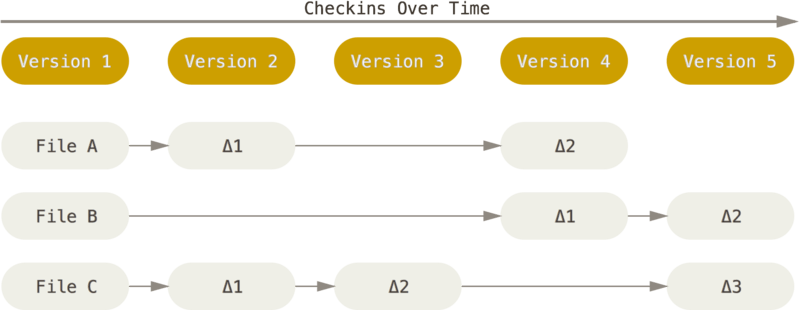
\includegraphics[width=0.8\linewidth]{figures/deltas}
  \end{center}
\end{frame}

\begin{frame}
  \frametitle{Snapshots, Not Differences}
  \begin{itemize}
   \item Git doesn’t think of or store its data this way. 
   \item Git thinks of its data more like a series of snapshots of a miniature filesystem. 
   \item Every time you commit, or save the state of your project, Git basically takes a picture of what all your files look like at that moment and stores a reference to that snapshot. 
   \item To be efficient, if files have not changed, Git doesn’t store the file again, just a link to the previous identical file it has already stored. 
   \item Git thinks about its data more like a \textbf{stream of snapshots}. 
  \end{itemize}
  
  \begin{center}
    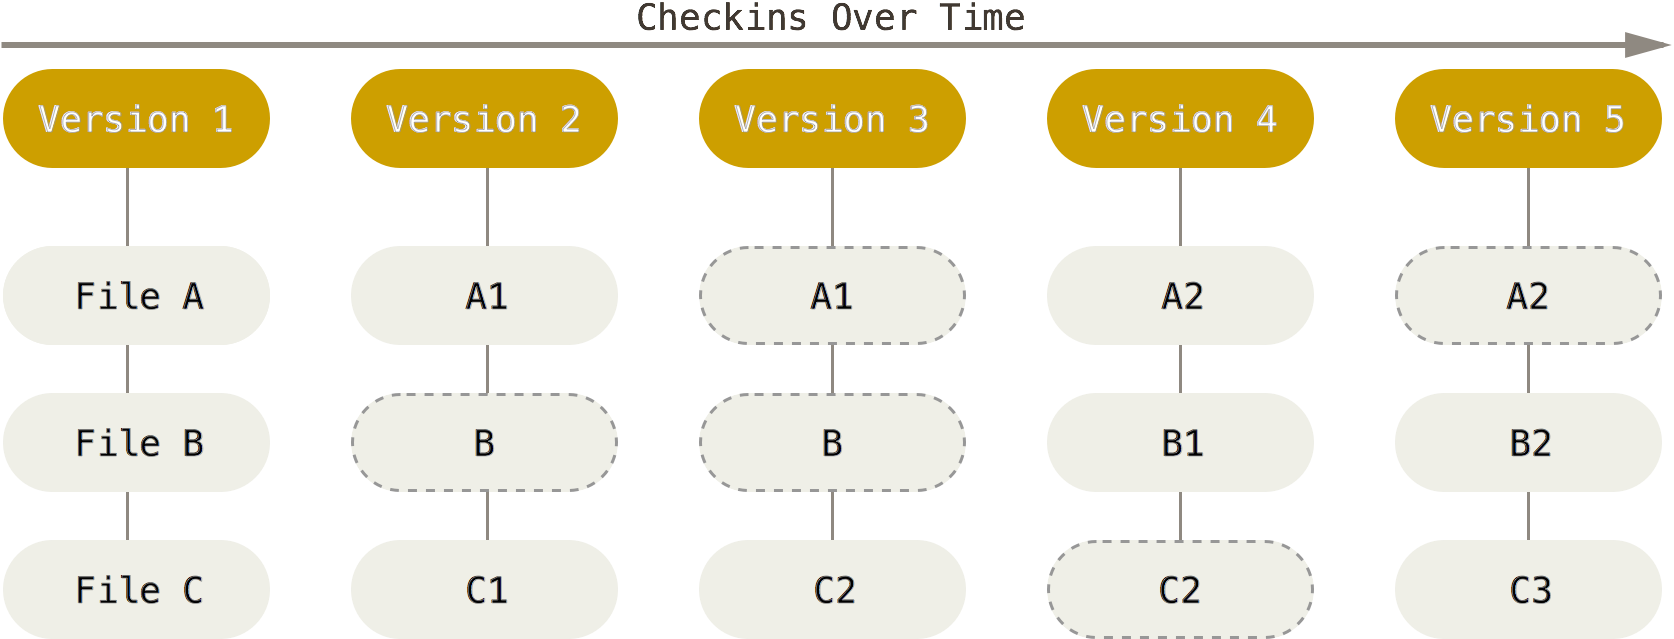
\includegraphics[width=0.8\linewidth]{figures/git-snapshots}
  \end{center}
\end{frame}



\begin{frame}
  \frametitle{Git}

  What is Git?

  \vspace{1em}

  Git is a distributed revision control system. It keeps \textbf{snapshots} of
  \textbf{the entirety} of your versioned directory through time using
  patches.

  \vspace{1em}

  \begin{center}
    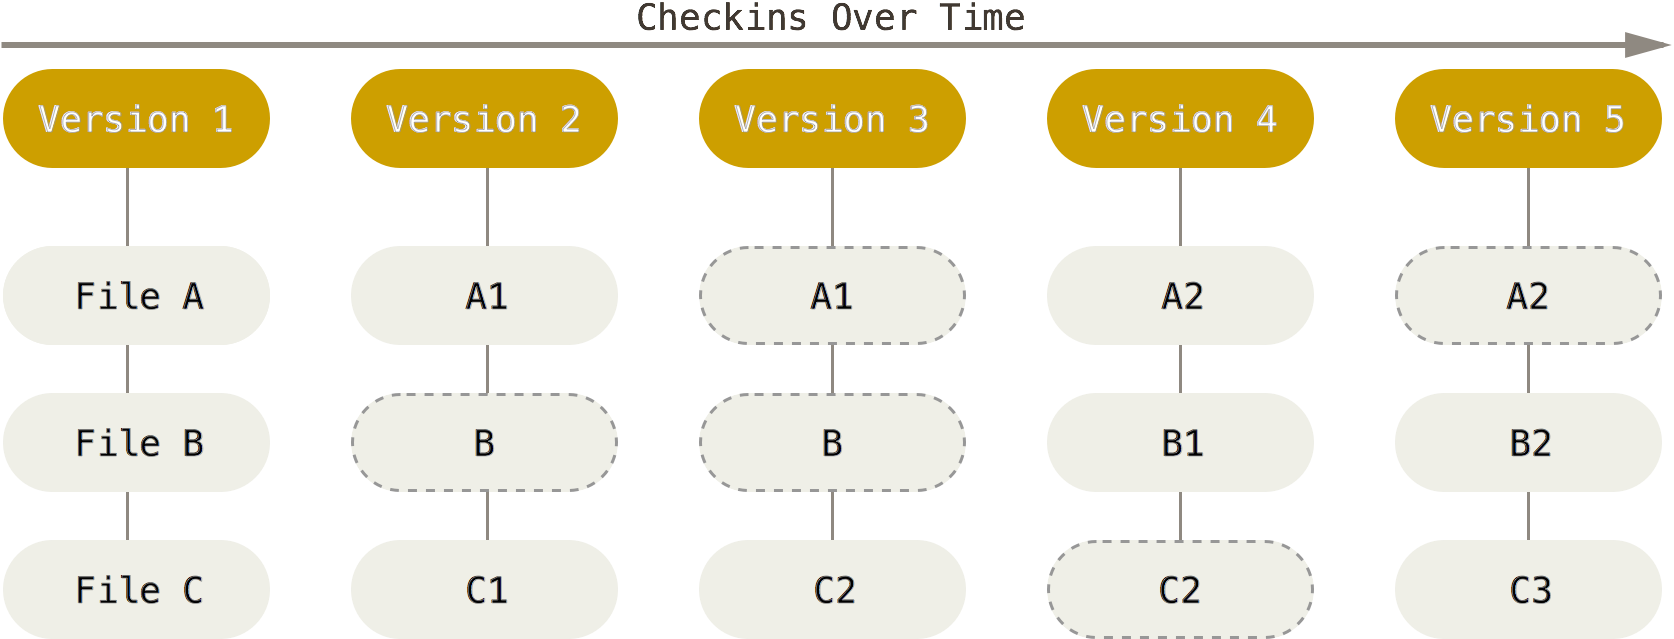
\includegraphics[width=0.8\linewidth]{figures/git-snapshots}
  \end{center}

  \only<2->{
    \begin{block}{Old tools, new usage}
      In order to create a snapshot, git uses \textit{diffs}, \textit{patches}
      and (SHA-1) \textit{hashes}
    \end{block}
  }

\end{frame}


\defverbatim[colored]\gitzeroone{
  \begin{textcode}
      file1.txt:                            file2.txt:

      I need to go to the store.            I need to go to the store.
      I need to buy some apples.            I need to buy some apples.
      When I get home, I'll wash the dog.   I also need to buy grated cheese.
                                            When I get home, I'll wash the dog.
  \end{textcode}
}

\defverbatim[colored]\gitzerotwo{
  \begin{shcode}
      $ diff file1.txt file2.txt > patch.txt
      $ cat patch.txt
      2a3
      > I also need to buy grated cheese.
  \end{shcode}
}

\begin{frame}
  \frametitle{\$h!tty situation!}

  \begin{center}
    
\includegraphics[width=0.6\linewidth]{figures/phdcomics}
  \end{center}

\end{frame}


\begin{frame}
  \frametitle{Diff/Patch}

  A \textit{diff} is a set of textual differences between files.

  \vspace{1em}

  \gitzeroone

  \vspace{1em}

  To create a \textit{patch}, use the \texttt{diff} command:

  \gitzerotwo

  \begin{exampleblock}{Translating}
    After line 2 in the first file, a line needs to be added: line 3 from the
    second file.
  \end{exampleblock}

\end{frame}


%*
\begin{frame}
  \frametitle{Applying patches (1)}

  Say you're receiving a \textit{diff} file, and you want to apply the changes. Do you know how to do it?
  \begin{itemize}
    \item You can do it manually (but what's the point?)
    \item You can use the command \textit{patch}
  \end{itemize}
  Let's say you wrote the following code:
  \includecode{codes_for_slides/cpu_usage.py}
  Then you noticed that there's something not correct so you asked a friend to help you!
\end{frame}

%*
\begin{frame}
  \frametitle{Applying patches (2)}

  Your friend sent you the following \textit{patch} file named \textit{cpu\_usage.diff}:
  \includecode{codes_for_slides/cpu_usage.diff}
  Do you notice what are the changes that your friend made? How to integrate them in your code?
\end{frame}

%*
\begin{frame}
  \frametitle{Applying patches (3)}

  To include the changes into your code \textit{cpu\_usage.py}, you can simply use the following command:
  \includebash{codes_for_slides/diff_cpu.sh}
  Then your code will be as follows:
  \includecode{codes_for_slides/cpu_usage1.py}
\end{frame}

\subsection{Hash}
\begin{frame}
  \frametitle{Hash}

  A (crypto) hash function is a function that can be used to map digital data
  of arbitrary size to a fixed length string, that is practically impossible to
  invert.

  \begin{center}
    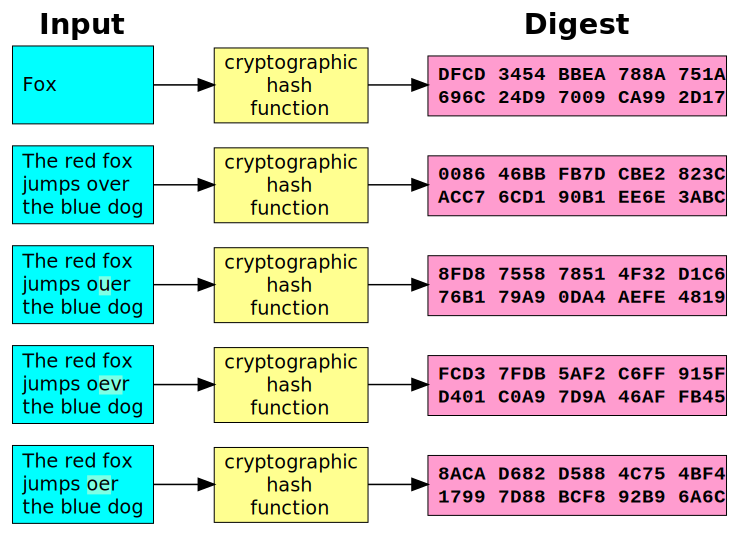
\includegraphics[width=0.6\linewidth]{figures/git-hash}
  \end{center}

  \vspace{1em}

  \textit{Notice that small changes on the input make the hash change a lot.}

\end{frame}


\begin{frame}
  \frametitle{Hash (collision)}

  \begin{block}{Nearly impossible to clash}
    It is nearly \textbf{impossible} that two natural sequences collide on the
    \textbf{same} repository.
  \end{block}

  \vspace{2em}

  If all world population would be developers and every one of them would
  commit to the \textbf{same} repository every second, the probability of 50\%
  collision would be reached in\footnote{http://diego.assencio.com/?index=eacd6eedf46c9dd596a5f12221ad15b8}:

  \[
    6.6 \times 10^6 \text{years}
  \]

\end{frame}

\subsection{Git states and workflow}

\begin{frame}
  \frametitle{Git states}

  Git contains 3 states for your project.

  \vspace{1em}

  \begin{center}
    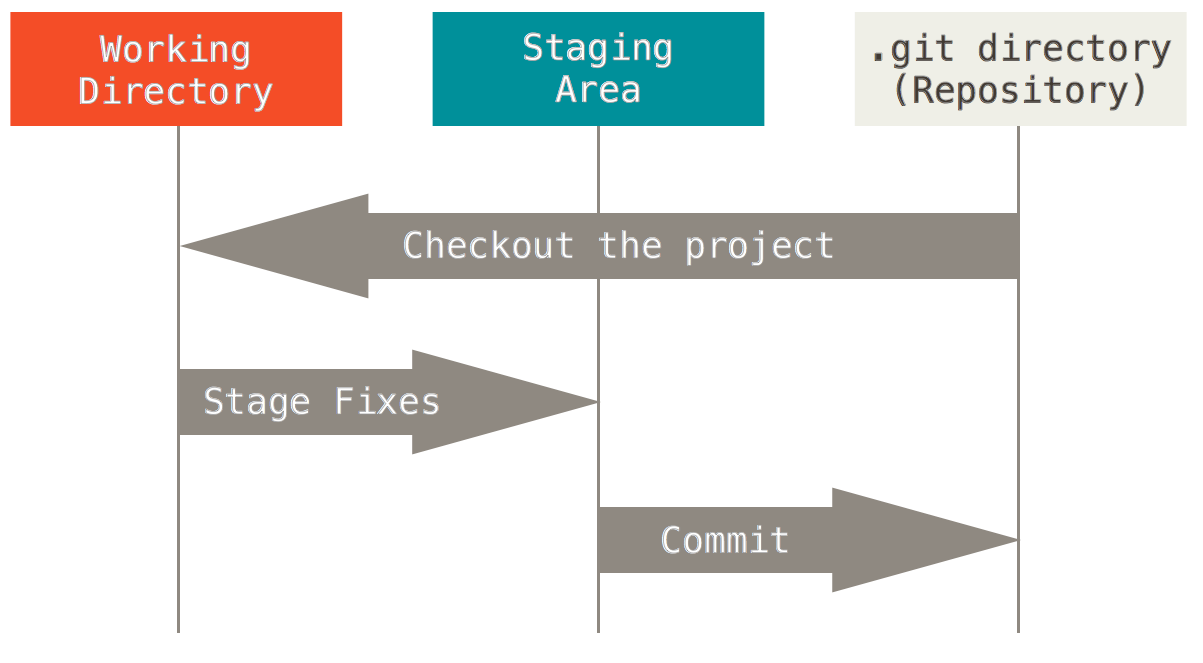
\includegraphics[width=0.9\linewidth]{figures/git-areas}
  \end{center}

\end{frame}


\begin{frame}

  \frametitle{Git workflow}

  Easy

  \vspace{2em}

  \begin{itemize}
    \item You modify files in your working directory.

    \item You stage the files, adding snapshots of them to your staging area.

    \item You do a commit, which takes the files as they are in the staging
      area and stores that snapshot permanently to your Git directory.
  \end{itemize}

\end{frame}

